\section{Usage Model}
\label{eval}

\begin{table*}[tb]
\centering
\begin{tabular}{|lrrr|}
\hline
TEST & Description Lines & Keys Collected & Transducer Lines \\
\hline
mdtest & 48 & 88 & 200 \\
ior & 45 & 101 & 143 \\
LANL fs\_test & 36 & 149 & 2 \\
\hline
\end{tabular}
\mycaption{eval-table}{Defining Experiments.}{
This table shows how many lines are necessary to describe typical parameter
sweeps for three different applications which are currently using \name\ at
LANL.  It also shows the number of \kv\ pairs collected from each \sub, and the
lines needed for the application-specific transducers which parse the output of
each \sub\ and produce these \kv\ pairs.  The LANL fs\_test transducer is so
small because LANL fs\_test already produces output in \kv\ format so that
transducer simply echoes its input to its output.  The other transducers are
larger because those applications do not have consistent output formatting so
every \kv\ must be parsed differently. 
}
\end{table*}


To use \name, a user first creates an experiment description file.  Because
\name\ handles both command generation and command dispatch automatically,
these description files need merely identify parameters and values of interest.
An example of such a file is shown in Figure~\ref{mdtest-desc}.  If the user
desires more than the default set of \kv\ pairs captured by \name, they can
additionally create an application-specific transducer.  Table~\ref{eval-table} 
lists the lines needed to create description files and transducers for
several applications currently using our framework.  

After defining descriptions and transducers, users can then begin to run their
experiments with the \dispatcher.  The user can optionally ask the \dispatcher\
to shuffle the \subs\ randomly before dispatching.  The value of this
randomness is shown in Figure~\ref{fig-random}.  By utilizing randomness, users
can more quickly see trends within their experiments than if the \subs\ are run
ordered by the parameter sweeps.  Note that utilizing randomness in this way is
not a new result nor is it our contribution.  Rather our contribution here is
that the \sub\ tracking and monitoring provided by \name\ allow randomness to
be exploited in this manner.  Without such simple tracking and monitoring, it
is much more difficult for the user to run \subs\ randomly; in the case of
interrupted experiments, naive resubmission will rerun previously completed
\subs\ and slow total time to completion for the experiment. 

As the \subs\ begin to complete, the user can track their progress with the
monitoring within \name, and can visualize the results with \dbviz.  The
following describes an example interactive session with \dbviz.

\begin{enumerate}
\item{The \dispatcher\ has already executed a set of \subs;
each \sub\ was executed ten times to provide
statistically meaningful results and variability measurements.  }
\item{The entire experiment was tagged with a \Term{description} of \Term{expr1}.}
\item{The transducer has collected general \kv\ pairs and has parsed specific
ones and has inserted them into a SQL server.}
\item{The user specifies "WHERE description like 'expr1'".}
\item{The user specifies the column \Term{numhosts} as the \xaxis\ 
and the column \Term{walltime} as the \yaxis.}
\item{The user asks to compare columns \Term{depth} and \Term{items} which
were the parameters swept and which the transducer parsed from the command
line.}
\item{\label{interactive-graph}A graph is created similar to that shown in Figure~\ref{dbviz-screen}.  The user 
notices unusually high variability and changes the display from lines to a 
scatter plot and discovers a few outliers. }
\item{Using outlier analysis,
the user pulls the complete row from the table for each outlier and
notices that some of the outliers were from \subs\ that did not complete
successfully.  To remove them from the analysis, the user adds a
successful \Term{retval} condition to the WHERE clause.}
\item{The user returns to linespoints mode but the variability still looks higher than expected.  The user queries the set of hidden differences and discovers
that data from multiple supercomputers with drastically different performance
characters has been combined.  The user then either adds \Term{system} to
the comparison fields or refines the filter to examine \subs\ from only a
single \Term{system}.}
\item{The user discerns that performance has degraded from previous 
experiments.  The user then combines multiple experiments and queries 
hidden differences again which reveals that \Term{osversion} has changed.
The user adds \Term{osversion} to the comparison fields and identifies that
as a reason for the performance degradation.
}
\end{enumerate}

A screenshot of \dbviz\ corresponding to step~\ref{interactive-graph} above is
shown in Figure~\ref{dbviz-screen}.  Notice that the key for the graph is 
constructed using each unique combination of the columns as specified in the
\Term{compare} field.  By default, these keys would read as \Term{k=v,k=v,...}
but using regular expressions in the Preferences panel (not shown) allows the
user to create semantically meaningful substitutions for \kv\ pairs.  For example, in this screenshot, the user has created a substitution to replace \Term{target=.*plfs.*} with \Term{PLFS-MNT}.

\begin{figure*}[tb]
  \centering
  \subfloat[\label{nonrandom}Ordered Dispatch]{
    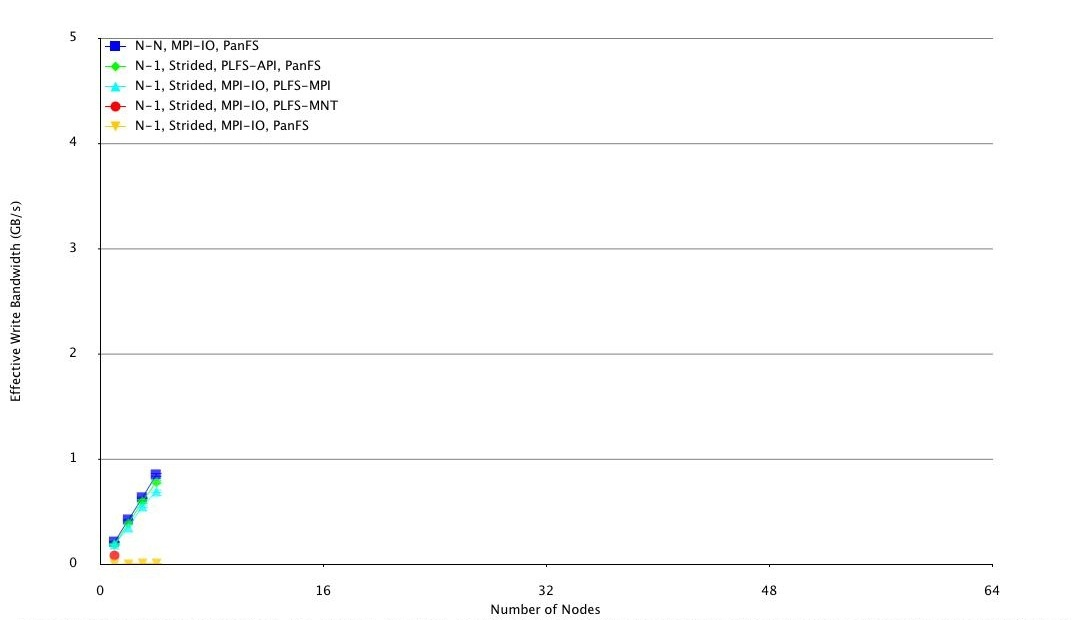
\includegraphics[width=0.3\textwidth,height=\figheight]{dbvizGraphsAndConfigs/pointsLTE4.jpg}
  }
  \subfloat[\label{random}Random Dispatch]{
    \includegraphics[width=0.3\textwidth,height=\figheight]{dbvizGraphsAndConfigs/random4Pts.jpg}
  }
  \subfloat[\label{random-full}Final Results]{
    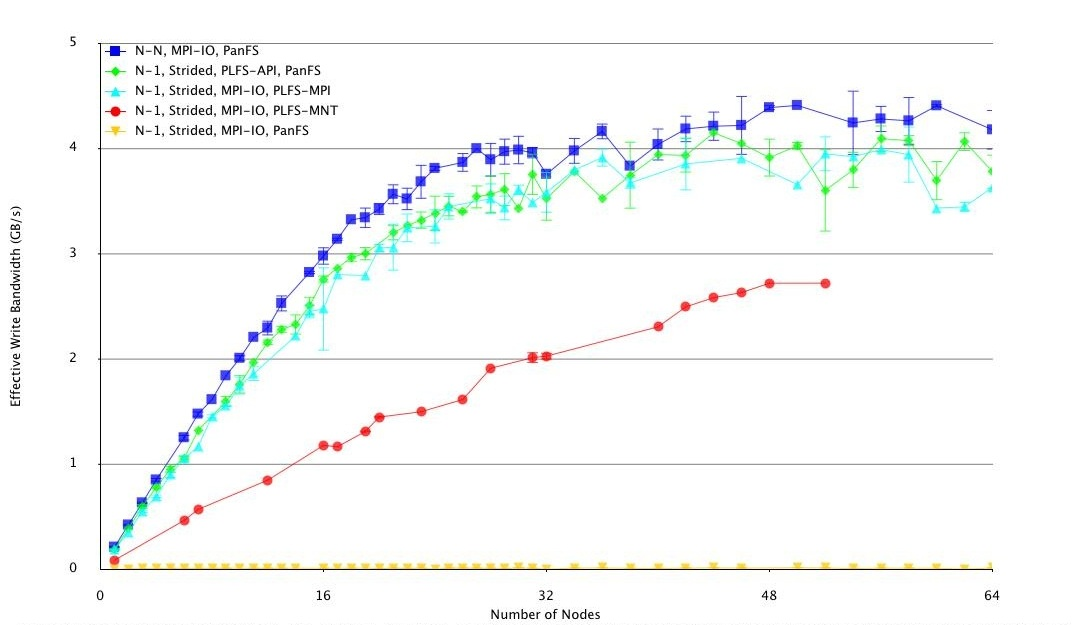
\includegraphics[width=0.3\textwidth,height=\figheight]{dbvizGraphsAndConfigs/allPoints.jpg}
  }
  \mycaption{fig-random}{Harnessing Randomness.}{
These three graphs illustrate the value of randomizing the generated commands
before dispatching them.  The graphs on the left and the middle were created
after only sixteen \subs\ were completed; the left-most is the graph produced when
the commands are dispatched in the order of their generation whereas the middle
graph was produced when the commands were randomly dispatched.  Finally, the
graph on the right shows the final results after all 492 \subs\ were completed.
By providing a much better approximation of the final graph, randomized 
commands allow computational steering much earlier in the experiment lifecycle.
}
\end{figure*}


